\begin{figure}[h]
\centering
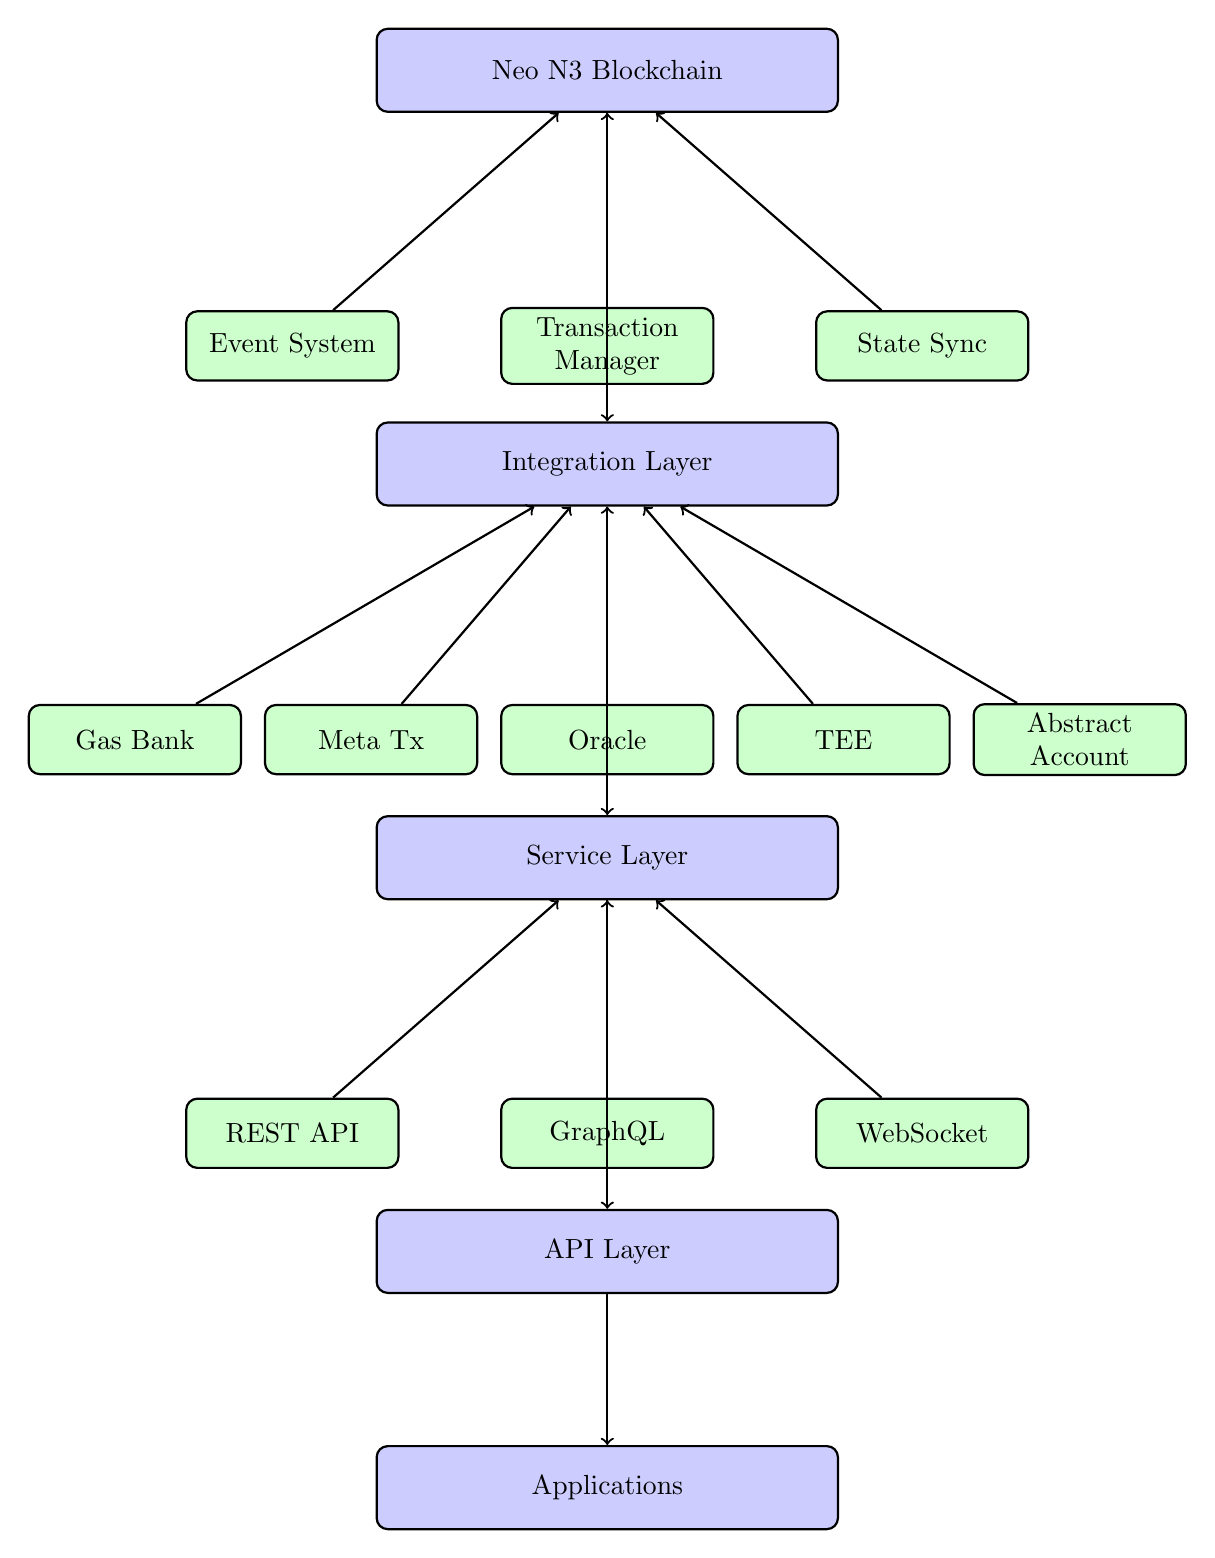
\begin{tikzpicture}[node distance=1.5cm, auto, thick]
    % Define styles
    \tikzstyle{layer} = [rectangle, draw, fill=blue!20, text width=16em, text centered, rounded corners, minimum height=3em]
    \tikzstyle{component} = [rectangle, draw, fill=green!20, text width=7em, text centered, rounded corners, minimum height=2.5em]
    \tikzstyle{line} = [draw, ->]
    
    % Place nodes - layers
    \node [layer] (blockchain) {Neo N3 Blockchain};
    \node [layer, below of=blockchain, node distance=5cm] (integration) {Integration Layer};
    \node [layer, below of=integration, node distance=5cm] (service) {Service Layer};
    \node [layer, below of=service, node distance=5cm] (api) {API Layer};
    \node [layer, below of=api, node distance=3cm] (app) {Applications};
    
    % Place nodes - components in Integration Layer
    \node [component, above of=integration, node distance=1.5cm, xshift=-4cm] (event) {Event System};
    \node [component, above of=integration, node distance=1.5cm] (tx) {Transaction Manager};
    \node [component, above of=integration, node distance=1.5cm, xshift=4cm] (state) {State Sync};
    
    % Place nodes - components in Service Layer
    \node [component, above of=service, node distance=1.5cm, xshift=-6cm] (gas) {Gas Bank};
    \node [component, above of=service, node distance=1.5cm, xshift=-3cm] (meta) {Meta Tx};
    \node [component, above of=service, node distance=1.5cm] (oracle) {Oracle};
    \node [component, above of=service, node distance=1.5cm, xshift=3cm] (tee) {TEE};
    \node [component, above of=service, node distance=1.5cm, xshift=6cm] (account) {Abstract Account};
    
    % Place nodes - components in API Layer
    \node [component, above of=api, node distance=1.5cm, xshift=-4cm] (rest) {REST API};
    \node [component, above of=api, node distance=1.5cm] (graphql) {GraphQL};
    \node [component, above of=api, node distance=1.5cm, xshift=4cm] (websocket) {WebSocket};
    
    % Draw edges between layers
    \path [line] (blockchain) -- (integration);
    \path [line] (integration) -- (service);
    \path [line] (service) -- (api);
    \path [line] (api) -- (app);
    
    % Connect components to layers
    \path [line] (event) -- (blockchain);
    \path [line] (tx) -- (blockchain);
    \path [line] (state) -- (blockchain);
    
    \path [line] (gas) -- (integration);
    \path [line] (meta) -- (integration);
    \path [line] (oracle) -- (integration);
    \path [line] (tee) -- (integration);
    \path [line] (account) -- (integration);
    
    \path [line] (rest) -- (service);
    \path [line] (graphql) -- (service);
    \path [line] (websocket) -- (service);
    
\end{tikzpicture}
\caption{Neo Service Layer Architecture}
\label{fig:architecture}
\end{figure}
